\chapter{UEFI, BIOS and platform}
\begin{note}[Abbreviations]:\\
	\begin{table}[h]
	\makegapedcells
	\centering
	\resizebox{\textwidth}{!}{%resizing the whole table
\begin{tabular}{|c|P{13cm}|}\hline
\textbf{Abbreviation} & \textbf{Meaning} \\  \hline

\href{https://en.wikipedia.org/wiki/Advanced_Configuration_and_Power_Interface}{\textbf{ACPI}} & Advanced Configuration and Power Interface \\   \hline
\href{https://en.wikipedia.org/wiki/Advanced_Programmable_Interrupt_Controller}{\textbf{APIC}} & Advanced Programmable Interrupt Controller \\   \hline
\href{https://en.wikipedia.org/wiki/Direct_memory_access}{\textbf{DMA}} & Direct Memory Access \\   \hline
\href{https://en.wikipedia.org/wiki/Direct_Media_Interface}{\textbf{DMI}} & Direct Media Interface \\   \hline
\href{https://en.wikipedia.org/wiki/EFI_system_partition}{\textbf{ESP}} & EFI System Partition \\   \hline
\href{https://www.dataman.com/media/datasheet/Intel/82802Ax.pdf}{\textbf{FWH}} & Firmware Hub \\   \hline
\href{https://en.wikipedia.org/wiki/GUID_Partition_Table}{\textbf{GPT}} & GUID Partition Table \\   \hline
\href{https://en.wikipedia.org/wiki/I/O_Controller_Hub}{\textbf{ICH}} & I/O Controller Hub (Southbridge)\\   \hline
\href{https://en.wikipedia.org/wiki/Industry_Standard_Architecture}{\textbf{ISA}} & Industry Standard Architecture\\   \hline
\href{https://en.wikipedia.org/wiki/Low_Pin_Count}{\textbf{LPC}} & Low Pin Count \\   \hline
\href{https://en.wikipedia.org/wiki/Northbridge_(computing)}{\textbf{MCH}} & Memory Controller Hub (Northbridge)\\   \hline
\href{https://en.wikipedia.org/wiki/Platform_Controller_Hub}{\textbf{PCH}} & Platform Controller Hub\\   \hline
\href{https://en.wikipedia.org/wiki/Conventional_PCI}{\textbf{PCI}} & Peripheral Component Interconnect\\   \hline
\textbf{PEIM} & Pre EFI Initialization Module\\   \hline
\href{https://en.wikipedia.org/wiki/System_Management_Bus}{\textbf{SMBus}} & System Management Bus \\   \hline
\href{https://en.wikipedia.org/wiki/System_Management_Mode}{\textbf{SMI}} & System Management Interrupt \\   \hline
\href{https://en.wikipedia.org/wiki/System_Management_Mode}{\textbf{SMM}} & System Management Mode \\   \hline
\href{https://en.wikipedia.org/wiki/Serial_Peripheral_Interface}{\textbf{SPI}} & Serial Peripheral Interface \\   \hline
\href{https://en.wikipedia.org/wiki/Trusted_Platform_Module}{\textbf{TPM}} & Trusted Platform Module \\   \hline
\href{https://www.uefi.org/}{\textbf{UEFI}} & Unified Extensible Firmware Interface \\   \hline
\end{tabular}
}
\caption{UEFI and platform abbreviations}
\end{table}

\end{note}
\section[GPT]{GPT\protect\footnote{GUID Partition Table}}
\begin{tabularx}{\textwidth}[t]{p{0.4\textwidth}rN}
 & \multirow{2}{*}{\includegraphics[scale=0.8]{Images/UEFI/GUIDPartitionTableScheme}} \\ 
 \begin{itemize}
 	\item GUID Partition Table (GPT) is a standard for the layout of the partition table on a physical storage device and it forms a part of the Unified Extensible Firmware Interface (UEFI) standard.
 	\item The GUID for an EFI system partition is C12A7328-F81F-11D2-BA4B-00A0C93EC93B
 	\item The Partition Entry Array describes partitions, using a minimum size of 128 bytes for each entry block.
 	\item Secondary GPT is nothing but a backup for Primary GPT
 \end{itemize} \\ [11cm]
\end{tabularx}

\begin{table}[h]
\begin{center}
	\begin{tabular}{|c|l|l|}\hline
		\multicolumn{1}{c}{ \bfseries Offset} & \multicolumn{1}{c}{\bfseries Length} & \multicolumn{1}{c}{\bfseries Contents} \\ \hline 
		0 (0x00) & 16 bytes & Partition type GUID \\ \hline
		16 (0x10)&	16 bytes&	Unique partition GUID\\ \hline
		32 (0x20)&	8 bytes&	First LBA (little endian)\\ \hline
		40 (0x28)&	8 bytes&	Last LBA (inclusive, usually odd)\\ \hline
		48 (0x30)&	8 bytes&	Attribute flags (e.g. bit 60 denotes read-only)\\ \hline
		56 (0x38)&	72 bytes&	Partition name (36 UTF-16LE code units)\\ \hline
	\end{tabular}
\end{center}
	\caption{GPT Entries}
\end{table}


\section{BIOS Flash Locations}
\begin{note}[Where bios is stored]
BIOS can reside in one of 3 locations:
\begin{itemize}
	\item Firmware Hub (FWH) (Old technology)
	\item SPI Flash (most likely this is the case)
	\item PCI (intended for debugging or recovering from a corrupted BIOS, not supported anymore on newer hardware)
\end{itemize}
\begin{center}
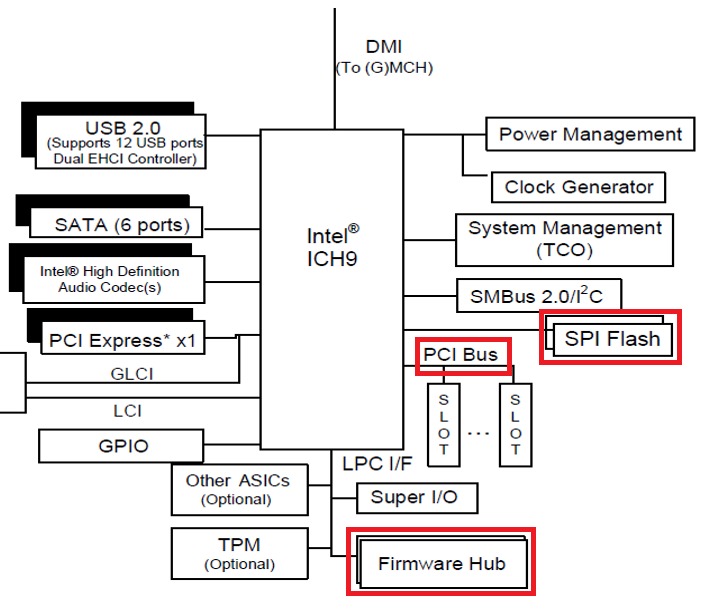
\includegraphics[scale=0.8]{Images/UEFI/BiosLocations}
\end{center}
\end{note}
\begin{note}[Find BIOS boot destination]:
	
To programmatically find where your BIOS is configured to boot from, you can view bits 11:10 in the General Control and Status Register (GCS). It is located at memory mapped offsets 3410-3413h in the Chipset Configuration Registers and Chipset Configuration Registers are mapped starting at the address held by RCBA\footnote{Root Complex Base Address Register}
\end{note}

\section{UEFI Firmware Volume}
\begin{note}[File types]:
\begin{lstlisting}[language=C]
typedef UINT8 EFI_FV_FILETYPE;

#define EFI_FV_FILETYPE_RAW                   0x01
#define EFI_FV_FILETYPE_FREEFORM              0x02
#define EFI_FV_FILETYPE_SECURITY_CORE         0x03
#define EFI_FV_FILETYPE_PEI_CORE              0x04
#define EFI_FV_FILETYPE_DXE_CORE              0x05
#define EFI_FV_FILETYPE_PEIM                  0x06
#define EFI_FV_FILETYPE_DRIVER                0x07
#define EFI_FV_FILETYPE_COMBINED_PEIM_DRIVER  0x08
#define EFI_FV_FILETYPE_APPLICATION           0x09
#define EFI_FV_FILETYPE_FIRMWARE_VOLUME_IMAGE 0x0b
#define EFI_FV_FILETYPE_FFS_PAD               0xf0
\end{lstlisting}
\end{note}
\section{System Management Mode}
\begin{note}[General notes]:
\begin{itemize}
	\item SMM is a special execution mode of IA-32 architecture that was introduced with i386, chapter 34 of \href{http://www.intel.com/content/www/us/en/processors/architectures-software-developer-manuals.html}{Intel 64 and IA-32 Architectures Software Developer’s Manual}
	\item Some time ago SMM was used by BIOS developers mostly for power management and legacy devices emulation, for example, PS/2 support (port 60h/64h) for USB keyboard and mouse. Nowadays it's also widely used for firmware and platform security purposes.
	\item SMM executable code and data lives inside SMRAM and when SMRAM is locked — it can't be accessed by code of operating system or user mode software. System firmware (legacy BIOS or UEFI) copies SMM code into SMRAM and locks it during platform initialization.
	\item Processor is switching to SMM only trough System Management Interrupt (SMI), it saving current execution context into SMRAM and start executing SMI handler that can exit from SMM and resume execution from saved context using RSM instruction.
	\item System Management Interrupt has the highest priority and can’t be masked. Most important facts about SMI handler execution environment:
	\begin{enumerate}
		\item Similar to 16-bit real address mode with paging disabled.
		\item CS segment base is SMRAM base, EIP is 8000h.
		\item Segment limits are set to 4 GBytes, you can switch to protected mode or long mode to access all of the physical memory.
		\item All I/O ports are available.
		\item SMM code can read or modify saved execution context.
		\item SMM code can set it’s own IDT and use software interrupts.
	\end{enumerate}
	\item There’s a several ways to generate SMI:
	\begin{enumerate}
		\item Ring 0 code can trigger software SMI at any time by writing some byte value to APMC I/O port B2h.
		\item Internal chipset registers (\verb|SMI_EN|, \verb|GEN_PMCON_1| and others) that accessible via PCI config space allows to enable or disable different kind of hardware SMI sources.
		\item You can route hardware interrupts into SMM by reconfiguring of advanced programmable interrupt controller (APIC) that integrated into CPU.
		\item I/O instruction restart CPU feature (chapter 34.12 of IA-32 Architectures Software Developer’s Manual) allows to generate SMI on any I/O port access by \verb|IN| or \verb|OUT| processor instruction.
	\end{enumerate}
	\item SMRAM can be located in Compatible Memory Segment (CSEG), High Memory Segment (HSEG) or Top of Memory Segment (TSEG) system memory regions.
\end{itemize}
\end{note}